\documentclass{article}
\usepackage{natbib}
\usepackage[labelfont=bf]{caption}
\usepackage{subcaption}
\usepackage{graphicx}
\usepackage{float}
\bibliographystyle{apalike}
\usepackage{lineno}
\linenumbers

\usepackage{geometry}
\geometry{letterpaper}
\geometry{margin=1in}

\usepackage{setspace}
\doublespacing
\captionsetup[figure]{font={stretch=2}}

\usepackage{authblk}
\usepackage{xcolor}

\newcommand{\matr}[1]{\mathbf{#1}}

\title{Efficient and Accurate Modeling of Flow through Dipping Aquifers with MODFLOW 6}

\author{
	Alden M. Provost, U.S. Geological Survey, Integrated Modeling and Prediction Division, U.S. Geological Survey, 12201 Sunrise Valley Dr, Reston, VA, USA  \\
	\and 
	Kerry Bardot, School of Earth Sciences, University of Western Australia, Perth, Australia \\
	\and 
	Christian D. Langevin, U.S. Geological Survey, Integrated Modeling and Prediction Division, 2280 Woodale Drive, Mounds View, MN, USA \\
	\and 
	James L. McCallum, School of Earth Sciences, University of Western Australia, Perth, Australia \\
	}


\date{\today}

\begin{document}

\maketitle

\textbf{Conflict of interest:} None.

\textbf{Key words:} groundwater flow simulation, discretization, dipping layers, cell connectivity, multi-point flux approximation, sedimentary structures

\textbf{Article impact statement: Groundwater flow through dipping aquifers can be accurately simulated using a vertically offset grid combined with an unstructured grid approach and the XT3D multi-point flow formulation in MODFLOW 6.}

\begin{abstract}
Groundwater flow through dipping hydrogeologic layers is often modeled with MODFLOW by specifying top and bottom elevations of model layers to coincide with top and bottom elevations of hydrogeologic layers.  With this approach, adjacent cells within a model layer are vertically offset from one another.  While the standard formulation in MODFLOW does not rigorously account for these offsets in the underlying flow calculations, results are generally expected to be accurate provided dip angles do not exceed $10^{\circ}$  {\color{red} (KB: I would remove this sentence as even 10 degrees if anisotropic say 10:1 is still  a 50\% error)}.  To improve the accuracy of flow simulations on unstructured grids, and to allow accurate simulation of arbitrarily oriented two- or three-dimensional anisotropy, the optional XT3D multi-point flow formulation was introduced in MODFLOW 6.  The XT3D flow formulation is designed to account for geometric irregularities in the grid, including vertical offsets between laterally adjacent cells, and to provide accurate results for both isotropic and anisotropic groundwater flow.  \cite{bardot2022} showed, however, that neither the standard formulation nor the XT3D formulation produced the correct flow direction and magnitude in simple tests involving flow through a steeply dipping, permeable hydrogeologic layer.  In this paper, we explain that the inability of XT3D to give accurate results in the steeply dipping test problem of \cite{bardot2022} was caused by the limited cell connectivity that is inherent in the most commonly used discretization packages in MODFLOW 6. The DIS and DISV discretization packages are based on layered connectivity in which cells have lateral connections only with cells in the same grid layer.  We demonstrate that layered lateral connectivity is insufficient to allow accurate simulation of flow through a steeply dipping hydrogeologic layer on a vertically offset grid.  When lateral connections between cells in adjacent grid layers are included using the fully unstructured (DISU) grid type, XT3D is able to calculate the flow magnitude and direction accurately for both isotropic and anisotropic conductivity oriented along the permeable hydrogeologic layer.  To realize this improved accuracy, the permeable hydrogeologic layer must be discretized vertically using at least two model layers. {\color{red} (AMP: Given the idealized nature of the test problem, how general can we be with our conclusions? I pulled it back here relative to what you had originally, CDL, but left a slightly stronger statement in the Conclusions, at least for now.})  Our findings suggest that, given appropriate discretization and cell connectivity, the combination of vertically offset grids with the XT3D flow formulation in MODFLOW 6 can provide a computationally efficient and accurate method for simulating flow through isotropic and anisotropic steeply dipping layers, a capability that was previously reserved to finite-element-based simulators. {\color{red} (AMP: Any Pal and Edwards-type MPFA stuff that's relevant to that final phrase? See also Conclusions)}

{\color{red} Here's another option for a simpler abstract! }

	
	Dipping aquifers are often modeled using a deformed grid whereby each hydrogeological layer is represented using a single grid layer. However, until the release of MODFLOW 6, accurate modeling of groundwater flow through dipping anisotropic layers has not been possible due to limitations of its finite difference conductance-based solution. The introduction of the XT3D multi-point flow formulation has allowed accurate simulation of the full conductivity tensor, as well as handling the flow solution for irregular cell geometries for unstructured grids. Through the use of a benchmark, \cite{bardot2022} showcased MODFLOW 6's capability to model flow through complex sedimentary structures, previously restricted to finite element simulators. However, the benchmark study also brought to light the inadequacy of the deformed vertically offset grid for accurate modeling of dipping layers, with or without XT3D. This paper explains that the limitation of the deformed grid is a result of poor cell connectivity between vertically adjacent model layers. Nonetheless, we also demonstrate that dipping layers may be efficiently and accurately modeled using a deformed vertically offset grid with full-connectivity, which can be achieved by combining MODFLOW 6's DISU discretization package with the XT3D flow formulation. A repeat benchmark study shows that this method produces accurate head and flux results in isotropic and anisotropic dipping layers, providing a minimum of two grid layers per hydrogeological layer are deployed which allows for sufficient vertical connectivity. 
	
\end{abstract}

\section{Introduction}

MODFLOW is commonly used to simulate groundwater flow in a wide variety of geological settings including sedimentary, alluvial and fractured rock aquifers \cite{modflow2005,Kumar2019}. Accurate simulation of the hydrostratigraphic sequences encountered in these geological settings requires that the model grid discretisation and solution technique can represent the scale and effects of important geologial features \cite{Reilly2004,bardot2022}, where permeability tensors are aligned along key structures \cite{hoaglund2003}. MODFLOW versions up to and including MODFLOW-2005 employ a structured grid based on a fixed number of layers, rows and columns \citep{modflow2005,modflow84,modflow88}. Further, through assuming that the hydraulic conductivity tensor aligns with the grid coordinates, the standard finite difference approximation can be applied accurately and efficiently to simulate groundwater flow \citep{modflow84}. The main trade-off in this approximation is that important hydrological and geological features are required to be mapped to the structured grids and orinetations need to be aligned to Cartesian coordinates. These requirements can result in pixelated features in plan view and, more significantly, create problems where geological layers are discontinuous at unconformities and faults, and where they are dipping and misaligned with the model grid \citep{bardot2022}. 

In meeting the requirements for the standard finite difference simulation, two methods have traditionally been used to represent dipping geological features in MODFLOW in versions up to and including MODFLOW-2005. One approach is to map the geological features to a rectilinear grid \citep{modflow84} in a method referred to as ‘grid overlay’  \citep{hoaglund2003}. Grid overlay preserves the control volume finite difference approximation but may require a high level of vertical discretization to accurately represent variable layering \citep{Zyvoloski2006}. An alternative approach is to set each hydrostratigraphic unit as its own model layer, resulting in 'deformed layers' \cite{anderson2015applied,Reilly2004} in a 'vertically offset' or 'conforming finite difference grid' \citep{Zyvoloski2006}. When the layers in the offset grid are not strictly horizontal and of a constant thickness, the standard finite difference approximation is violated \citep{Zheng1994,anderson2015applied,Reilly2004}. To maintain a reasonable level of accuracy, \cite{anderson2015applied} recommend a $10^{\circ}$ dip as a practical upper limit for using vertical offsets.

The capability to represent complex ‘un-layered’ geology using unstructured grids was developed in versions of MODFLOW after MODFLOW 2005, namely MODFLOW-USG \citep{modflowusg} and MODFLOW 6 \citep{modflow6software}. Unstructured versions offered greater flexibility in representing the shape of geological features in plan view. To overcome the violations of the control volume finite difference approximations bought about by unsturctured grids, Ghost Node corrections were implemented in MODFLOW-USG \citep{modflowusg}, with MODFLOW 6 incorporating the XT3D option, which solves the full tensorial version of Darcy’s law \citep{modflow6xt3d}. Two of the discretisation options in MODFLOW 6 (known as the DIS and DISV options) preserve the layered connectivity approach from earlier MODFLOW versions \citep{modflow6framework}; however, both MODFLOW-USG, and the DISU option within MODLFOW 6 offer the capability to hydraulically connect multiple cells horizontally to the same face using the vertically staggered option with full connectivity, hence revolutionising the traditional layered-approach. We note that this type of connection is not implicit within the unstructured versions of the code, but needs to be defined by the user.

Recently Bardot et al. (2022) revisited the capacity of MODFLOW 6 to represent non-orthogonal geologic structures. A simple test problem was created using a highly conductive channel misaligned with a Cartesian grid in both plan and transect to test the code's capability to solve flow using flexible gridding in plan, and dipping anisotropic conductivity in transect. Through comparison with an analytical solution, the authors demonstrated that the application of XT3D produced excellent results in plan view with flexible gridding, highlighting the improved capabilities of MODFLOW 6. However, when attempting to represent an analytically identical problem in transect view, the authors experienced large errors in flow magnitudes and directions when using a vertically offset grid both with and without the use of XT3D. They recommended the use of the grid overlay method in conjunction with XT3D for simulating steeply dipping layers. A preliminary analysis by two authors of the present work (Provost and Langevin) hypothesized that the limited cell connectivity offered by the vertically offset grid was inadequate for allowing an accurate flow solution as it does not consider full connectivity between the offset layers.

Although the grid overlay method accurately simulates groundwater flow in dipping layers, the high vertical resolution required to represent geological structure becomes increasingly significant as dip increases, making the solution computationally prohibitive in some cases due to the large number of cells. This paper investigates the limitations of vertically offset grids and develops a solution for accurate and efficient grid representation in the vertical direction. We present a theoretical background which explains in detail the connectivity issues associated with vertically distorted grids, and propose a method to upgrade its accuracy using full connectivity grids together with XT3D option. The effectiveness of the proposed approach is validated through the benchmark problem of \cite{bardot2022}. Finally, we discuss the implications of our findings for practical groundwater problems involving steeply dipping hydrogeologic layers.

\section{Theoretical Background}

\begin{figure}
	\begin{center}
	\includegraphics[scale=0.6]{../figures/schem_conn_area_flux.png}
	\caption{Schematics showing (a) cell connectivity and (b) cell-cell interface fluxes in a two-grid-layer model of a dipping hydrogeologic layer. Hatching denotes impermeable boundaries along the top and bottom of the hydrogeologic layer. In (a), black circles represent cell centers. Blue lines represent hydraulic connections between cells in a layered-connectivity grid. Red lines represent additional connections that must be made to achieve full connectivity. In (b), gray arrows represent the uniform groundwater flux the model is attempting to simulate. Blue arrows represent components of the uniform groundwater flux normal to the horizontal and vertical cell-cell interfaces in the layered-connectivity grid. Red arrows represent components of the uniform groundwater flux normal to the additional vertical cell-cell interfaces introduced to represent the full connectivity.}
	\label{fig:schem-conn-area-flux}
	\end{center}
\end{figure}

Figure \ref{fig:schem-conn-area-flux}a shows a group of four cells in a two-grid-layer, cross-sectional MODFLOW 6 model of fully saturated flow through a permeable hydrogeologic layer (aquifer) with impermeable top and bottom boundaries. The cells have horizontal tops and bottoms and can therefore follow the dip of the hydrogeologic layer only on average. If the grid is represented using a layered grid type (DIS or DISV) in MODFLOW 6, a cell is hydraulically connected to each adjacent cell in the same grid layer, regardless of whether or not the cells overlap, and with each overlying and underlying cell, as indicated by the blue lines that connect cell centers in Figure \ref{fig:schem-conn-area-flux}a. In this work we call this a vertically offset grid with ``layered connectivity.''  Note that cells that have overlapping vertical faces but are in different grid layers (e.g., cells 1A and 2B) do not have a direct hydraulic connection in a grid with layered connectivity. The addition of such connections between cells in different grid layers, as indicated by the red lines that connect cell centers in Figure \ref{fig:schem-conn-area-flux}a, results in a grid with ``full connectivity.''  In MODFLOW 6, only layered connectivity can be represented in structured (DIS) and vertex-based (DISV) grids. Fully unstructured (DISU) grids allow representation of any kind of cell connectivity, including layered or full connectivity.

The default method for representing the flow between two hydraulically connected model cells in MODFLOW 6 is the ``conductance-based flow formulation'' \citep{modflow6gwf}. In this formulation, which is based on the commonly used two-point flux approximation which arises from the starndard finite difference formulation \citep{modflow84}, the flow is proportional to the difference in the hydraulic heads computed at the two cell centers and a hydraulic conductance based on an effective hydraulic conductivity for the connection between the cells. On strictly rectilinear grids, such as structured MODFLOW grids with no vertical offset between cells in the same grid layer, and hydraulic conductivity that is isotropic or has anisotropy aligned with the three mutually perpendicular grid directions, the conductance-based formulation is second-order accurate \citep{dehotin2010modeling, modflow6gwf}. This is because strictly rectilinear grids satisfy the ``control-volume finite-difference (CVFD) requirement'' that the straight-line connection between two cell centers must intersect the midpoint of the cell-cell interface at a right angle \citep{narasimhan1976integrated}. However, vertically offset grids violate the CFVD requirement because nominally ``horizontal'' connections between cell centers in the same grid layer are not strictly horizontal and therefore not perpendicular to the vertical cell-cell interfaces they intersect. For example, in Figure \ref{fig:schem-conn-area-flux}a, the connection between cells 1A and 1B is not perpendicular to the cell-cell interface, which compromises the accuracy of the conductance-based formulation.

The conductance-based formulation was the only flow formulation available in versions of MODFLOW prior to MODFLOW 6. As mentioned earlier, the limitations of the conductance-based formulation on vertically offset grids were well recognized. However, the ability to use unstructured grids in MODFLOW-USG and MODFLOW 6 introduced new ways to violate the CVFD requirement, and thereby render the conductance-based formulation less accurate, even in the absence of vertical offsets. The concept of a ``ghost node'' was included in MODFLOW-USG \citep{modflowusg}, and subsequently in MODFLOW 6, as a simple and optional way to improve the accuracy for grids that violated the CVFD requirement.  However, implementation of the ghost-node correction is highly problem dependent, and it is not obvious how to specify optimal ghost-node locations and weights on complex, unstructured grids.  As a more ``automatic'' alternative to the ghost-node method for improving accuracy, and as a way to allow accurate simulation of arbitrarily oriented two- or three-dimensional anisotropy, the optional XT3D flow formulation \citep{modflow6xt3d} was introduced in MODFLOW 6.  XT3D formulates the flow between two cells by interpolating head values from the two cells and their neighboring cells to construct an estimate of the full, two- or three-dimensional head-gradient vector on each side of the cell-cell interface; applying the cell conductivity tensors to obtain an estimate of the groundwater flux  normal to the interface on each side of the interface; and reconciling the two flux estimates to ensure continuity of flow across the interface. By performing flow calculations using Darcy's Law in its tensorial form, based on a ``multi-point'' approximation of the head gradient, XT3D accounts for both arbitrarily oriented anisotropy and geometric irregularity of the grid.

The dipping-hydrogeologic-layer benchmark problem of \cite{bardot2022} used a vertically offset layered grid, which is the type of grid used most often in MODFLOW models. Test simulations using the conductance-based flow formulation for a steeply dipping hydrogeologic layer (which we will call the ``aquifer'') embedded in a near-impermable domain yielded significant errors in the simulated flows. The simulated groundwater flux in the middle of the aquifer was not along the $30^{\circ}$ incline of the aquifer as expected, but nearly horizontal ($0.03^{\circ}$ incline), and its magnitude was overestimated by 15\%. Significant errors in the simulated flows were expected in this case, given that the conductance-based flow formulation does not rigorously account for violations of the CVFD requirement that the cell-cell connection be perpendicular to the cell-cell interface, and that it takes the connection length to be the horizontal distance between cell centers.  Given the ability of XT3D to account rigorously for cell connections that are not perpendicular to cell-cell interfaces, and for the increase in connection length due to the slope of the connection, rerunning the simulation with XT3D activated could have been expected to improve the flow solution substantially. However, \cite{bardot2022} observed similarly poor results with XT3D: the flux was still nearly horizontal ($0.01^{\circ}$ incline), and its magnitude was overestimated by 12\%. Based on a preliminary analysis by two authors of the present work (Provost and Langevin), \cite{bardot2022} hypothesized that the unexpectedly large error in the flow solution with XT3D was related to inadequate cell connectivity.

The role of cell connectivity in enabling accurate simulation of flow along a dipping hydrogeologic layer can be understood by considering Figure \ref{fig:schem-conn-area-flux}b. Components of the groundwater flux (specific discharge) vector are displayed on each cell-cell interface and are representative of steady, uniform flow along the hydrogeologic layer. Gray vectors represent the uniform flux oriented along the hydrogeologic layer, which the model is attempting to simulate. Blue vectors represent the flux components normal to cell-cell interfaces that correspond to blue connections in Figure \ref{fig:schem-conn-area-flux}a, which are common to both the layered-connectivity and full-connectivity grids. Red vectors represent the flux components normal to cell-cell interfaces that correspond to red connections in Figure \ref{fig:schem-conn-area-flux}a, which are lacking in the layered-connectivity grid.

The blue vectors in Figure \ref{fig:schem-conn-area-flux}b show that to simulate steady, uniform flow along the dipping hydrogeologic layer, cells must exchange water not only ``horizontally'' with neighboring cells in the same grid layer, but also vertically with cells in the adjacent grid layer. Specifically, there must be flow from cells in the bottom grid layer to cells in the top grid layer, which corresponds to the vertical component of the groundwater flux. Note, however, that the blue vectors alone are incompatible with steady, uniform flow along the hydrogeologic layer because the exchange of water between the two grid layers is in one direction only: upward. Such a steady-state flow configuration would imply continuous depletion of flow within the bottom grid layer and accumulation of flow within the top grid layer as one moves along the hydrogeologic layer in the direction of flow. Thus, steady, uniform flow along the hydrogeologic layer cannot be simulated accurately without some mechanism for returning flow from the top grid layer to the bottom grid layer. The full-connectivity grid provides such a mechanism by offering additional connections between cells in adjacent grid layers. Vertical flows from the bottom grid layer to the top grid layer, represented by vertical blue vectors in Figure \ref{fig:schem-conn-area-flux}b, can be returned to the bottom grid layer by nominally ``horizontal'' flows, represented by red vectors in Figure \ref{fig:schem-conn-area-flux}b. Although this concept has been illustrated using a two-grid-layer model for simplicity, the same reasoning applies given any number of grid layers.

Once the full connectivity is established, it is the role of the flow formulation to account properly for the geometry of the grid, a task for which XT3D was specifically designed. However, XT3D alone cannot compensate for cell connectivity that does not provide adequate pathways for flow. This explains why using XT3D did not improve the simulation results substantially on the layered-connectivity grid in the benchmark tests of \cite{bardot2022}.  In the middle section of the hydrogeologic layer, away from the end boundary conditions, the flow solution approached steady, uniform flow the only way that it could given the limited connectivity: by suppressing vertical flows between grid layers, thereby rendering the overall flow approximately horizontal.

The arguments presented in this section suggest that, in addition to the use of XT3D, full connectivity can be important for obtaining an accurate flow solution in MODFLOW 6 simulations that involve steeply dipping hydrogeologic layers. The next section presents results of simulations designed to test this hypothesis.

\section{Description of Test Problem}

The test problem is patterned after the cross-sectional (transect) benchmark of \cite{bardot2022}. It attempts to simulate uniform flow in an inclined permeable hydrogeologic layer (``aquifer'') embedded in less permeable material (the ``domain'').

To simulate flow along an aquifer of uniform thickness inclined at angle $\theta$ relative to the horizontal ($30^{\circ}$ for the base case), heads are specified at the centers of cells along the perimeter of the model using a formula that corresponds to a uniform, unit head gradient:
\begin{equation}
\label{eqn:head_analyt_along}
h = - x \cos \theta - z \sin \theta.
\end{equation}

\noindent where $h$ is head in meters and $x$ and $z$ are the horizontal and vertical model coordinates, respectively, in meters. The hydraulic conductivity of the aquifer is set to 1 m/d (meter per day) so that the analytical flow solution is a groundwater flux of 1 m/d along the aquifer. In the base case, the conductivity of the domain surrounding the aquifer is set to $10^{-6}$ m/d to effectively isolate the aquifer hydraulically.

Two methods of discretization are used to simulate the test problem: (1) vertically offset grid of the MODFLOW 6 DIS (structured) type, and (2) vertically offset grid of MODFLOW 6 DISU (unstructured) type. The cell geometry in these two discretization methods is identical, but the cell connectivity is different. The DIS grid uses layered connectivity, and the DISU grid includes the additional connections between cells in adjacent grid layers needed to realize full connectivity. The DISU grid is constructed by starting with a DIS grid, converting it to an equivalent DISU grid, and then implementing full connectivity. The base case uses grids consisting of 11 columns and 9 layers of cells, with 3 layers within the aquifer, 3 layers in the domain above the aquifer, and 3 layers in the domain below the aquifer.  The model width was set to 11 m such that each column was 1m wide. Cells within the aquifer were chosen to stay square (i.e. 1 x 1 m) for the purpose of the test problem to eliminate distortion effects. Corner cells in the lower left and upper right corner were also set to be the same dimension as the aquifer cells. The resulting base model vertical height is 14.77 m.  

The above description represents the base-case test problem. However, the results also include simulations designed to investigate the effects of varying the gridding resolution, the dip angle of the aquifer, the conductivity contrast between the aquifer and the domain, and the anisotropy of the conductivity tensor.

Jupyter notebooks created for the test problem are available in the Supporting Information that accompanies this paper. The notebooks leverage the capabilities of FloPy \citep{bakker2016scripting, hughes2023flopy} to assist in setting up input for and processing results from the MODFLOW 6 simulations. A Python script for converting structured, DIS grids to unstructured, DISU grids with full connectivity is included.

\section{Results and Discussion}

To demonstrate the effect of cell connectivity on the accuracy of simulated flow through a steeply dipping hydrogeologic layer (aquifer), results for the base case described in the previous section are compared for simulations that use either layered or full connectivity, and either the standard or the XT3D flow formulation. The base case is then modified to further investigate the effects of grid resolution, aquifer dip angle, conductivity contrast between the aquifer and the surrounding domain, and anisotropic hydraulic conductivity.

Plots of specific discharge (groundwater flux) at cell centers and flows across cell-cell interfaces (face flows) calculated by MODFLOW 6 are used to illustrate the accuracy of the simulated flows. The magnitude and direction of specific discharge at the cell in the center of the aquifer, at which boundary effects are presumably minimized, and the total volumetric flow rate entering the aquifer through the left-hand boundary, which consists of constant-head (CHD) cells, are also reported as ``representative'' values of flow. Maximum head errors are also reported for the base case.

Specific discharge at cell centers is calculated in a postprocessing step using distance-weighted interpolation of face flows calculated by MODFLOW 6 and reported in the binary budget output file. For the purpose of illustrating and evaluating the results of this idealized benchmark, specific discharge in cells within the aquifer is calculated using only face flows between cells within the aquifer. Likewise, specific discharge in cells within the surrounding domain is calculated using only face flows between cells within the domain. Specific discharge values reported in the binary budget output file by MODFLOW 6 are different than the values reported here for cells that are adjacent to the boundary between the aquifer and the domain. This is because MODFLOW interpolates specific discharge in a cell using all of the face flows for that cell, including flows across cell faces on the aquifer-domain boundary. Those flows represent an ``average'' of the different flows on either side of the aquifer-domain boundary. Therefore, specific discharge calculated in a cell adjacent to the aquifer-domain boundary is affected by the different flow rate on the other side of the boundary. While this is an unavoidable consequence of vertically offset discretization in practical applications, and not necessarily a problem, users should be aware of these effects when interpreting the results of MODFLOW 6 dispersive-transport and MODPATH particle-tracking simulations.

\subsection{Effects of Cell Connectivity and Flow Formulation}

The numerical solution for the layered connectivity grid confirms the findings of \cite{bardot2022} in that fluxes are predominantly horizontal (top row, Figure \ref{fig:fig2}). We see that despite an enforced hydraulic gradient of $30^{\circ}$, the vertical component of the flux cannot propagate through the aquifer given that cells along the aquifer top are hydraulically disconnected from the low permeability domain, hence forcing flow horizontally (red arrows on right panel). The numerical solution for this grid type is a problem of cell connectivity, and thus the XT3D formulation does not resolve this issue (second row, Figure \ref{fig:fig2}). Results for the full-connectivity grid with the standard conductance-based formulation shows an improvement in the flow solution (third row, Figure \ref{fig:fig2}), with the XT3D formulation successfully reproducing the analytical solution (bottom row, Figure \ref{fig:fig2}). We see that the grid with full connectivity allows incorporation of the vertical flow component, thus permitting cross-connection between grid layers.

The results shown in Figure \ref{fig:fig2}a and b , which are based on a vertically offset grid with layered connectivity, are consistent with the findings of \cite{bardot2022}. Despite boundary heads designed to induce specific discharge of 1 m/d along the $30^{\circ}$ incline of the aquifer, the simulated flow within the aquifer is predominantly horizontal, and the magnitude of the specific discharge at the center of the aquifer and the total flow entering the aquifer are both overestimated. The XT3D flow formulation is unable to compensate for the inadequate cell connectivity (Figure \ref{fig:fig2}b), which does not allow flow between laterally adjacent cells in different grid layers.

The vertically offset grid with full connectivity (Figure \ref{fig:fig2}c and d) show significantly improved results, even for the standard flow formulation (Figure \ref{fig:fig2}c). Using the XT3D flow formulation provides the most accurate results, as expected (Figure \ref{fig:fig2}d).

\begin{figure}[p!]
	\begin{center}
	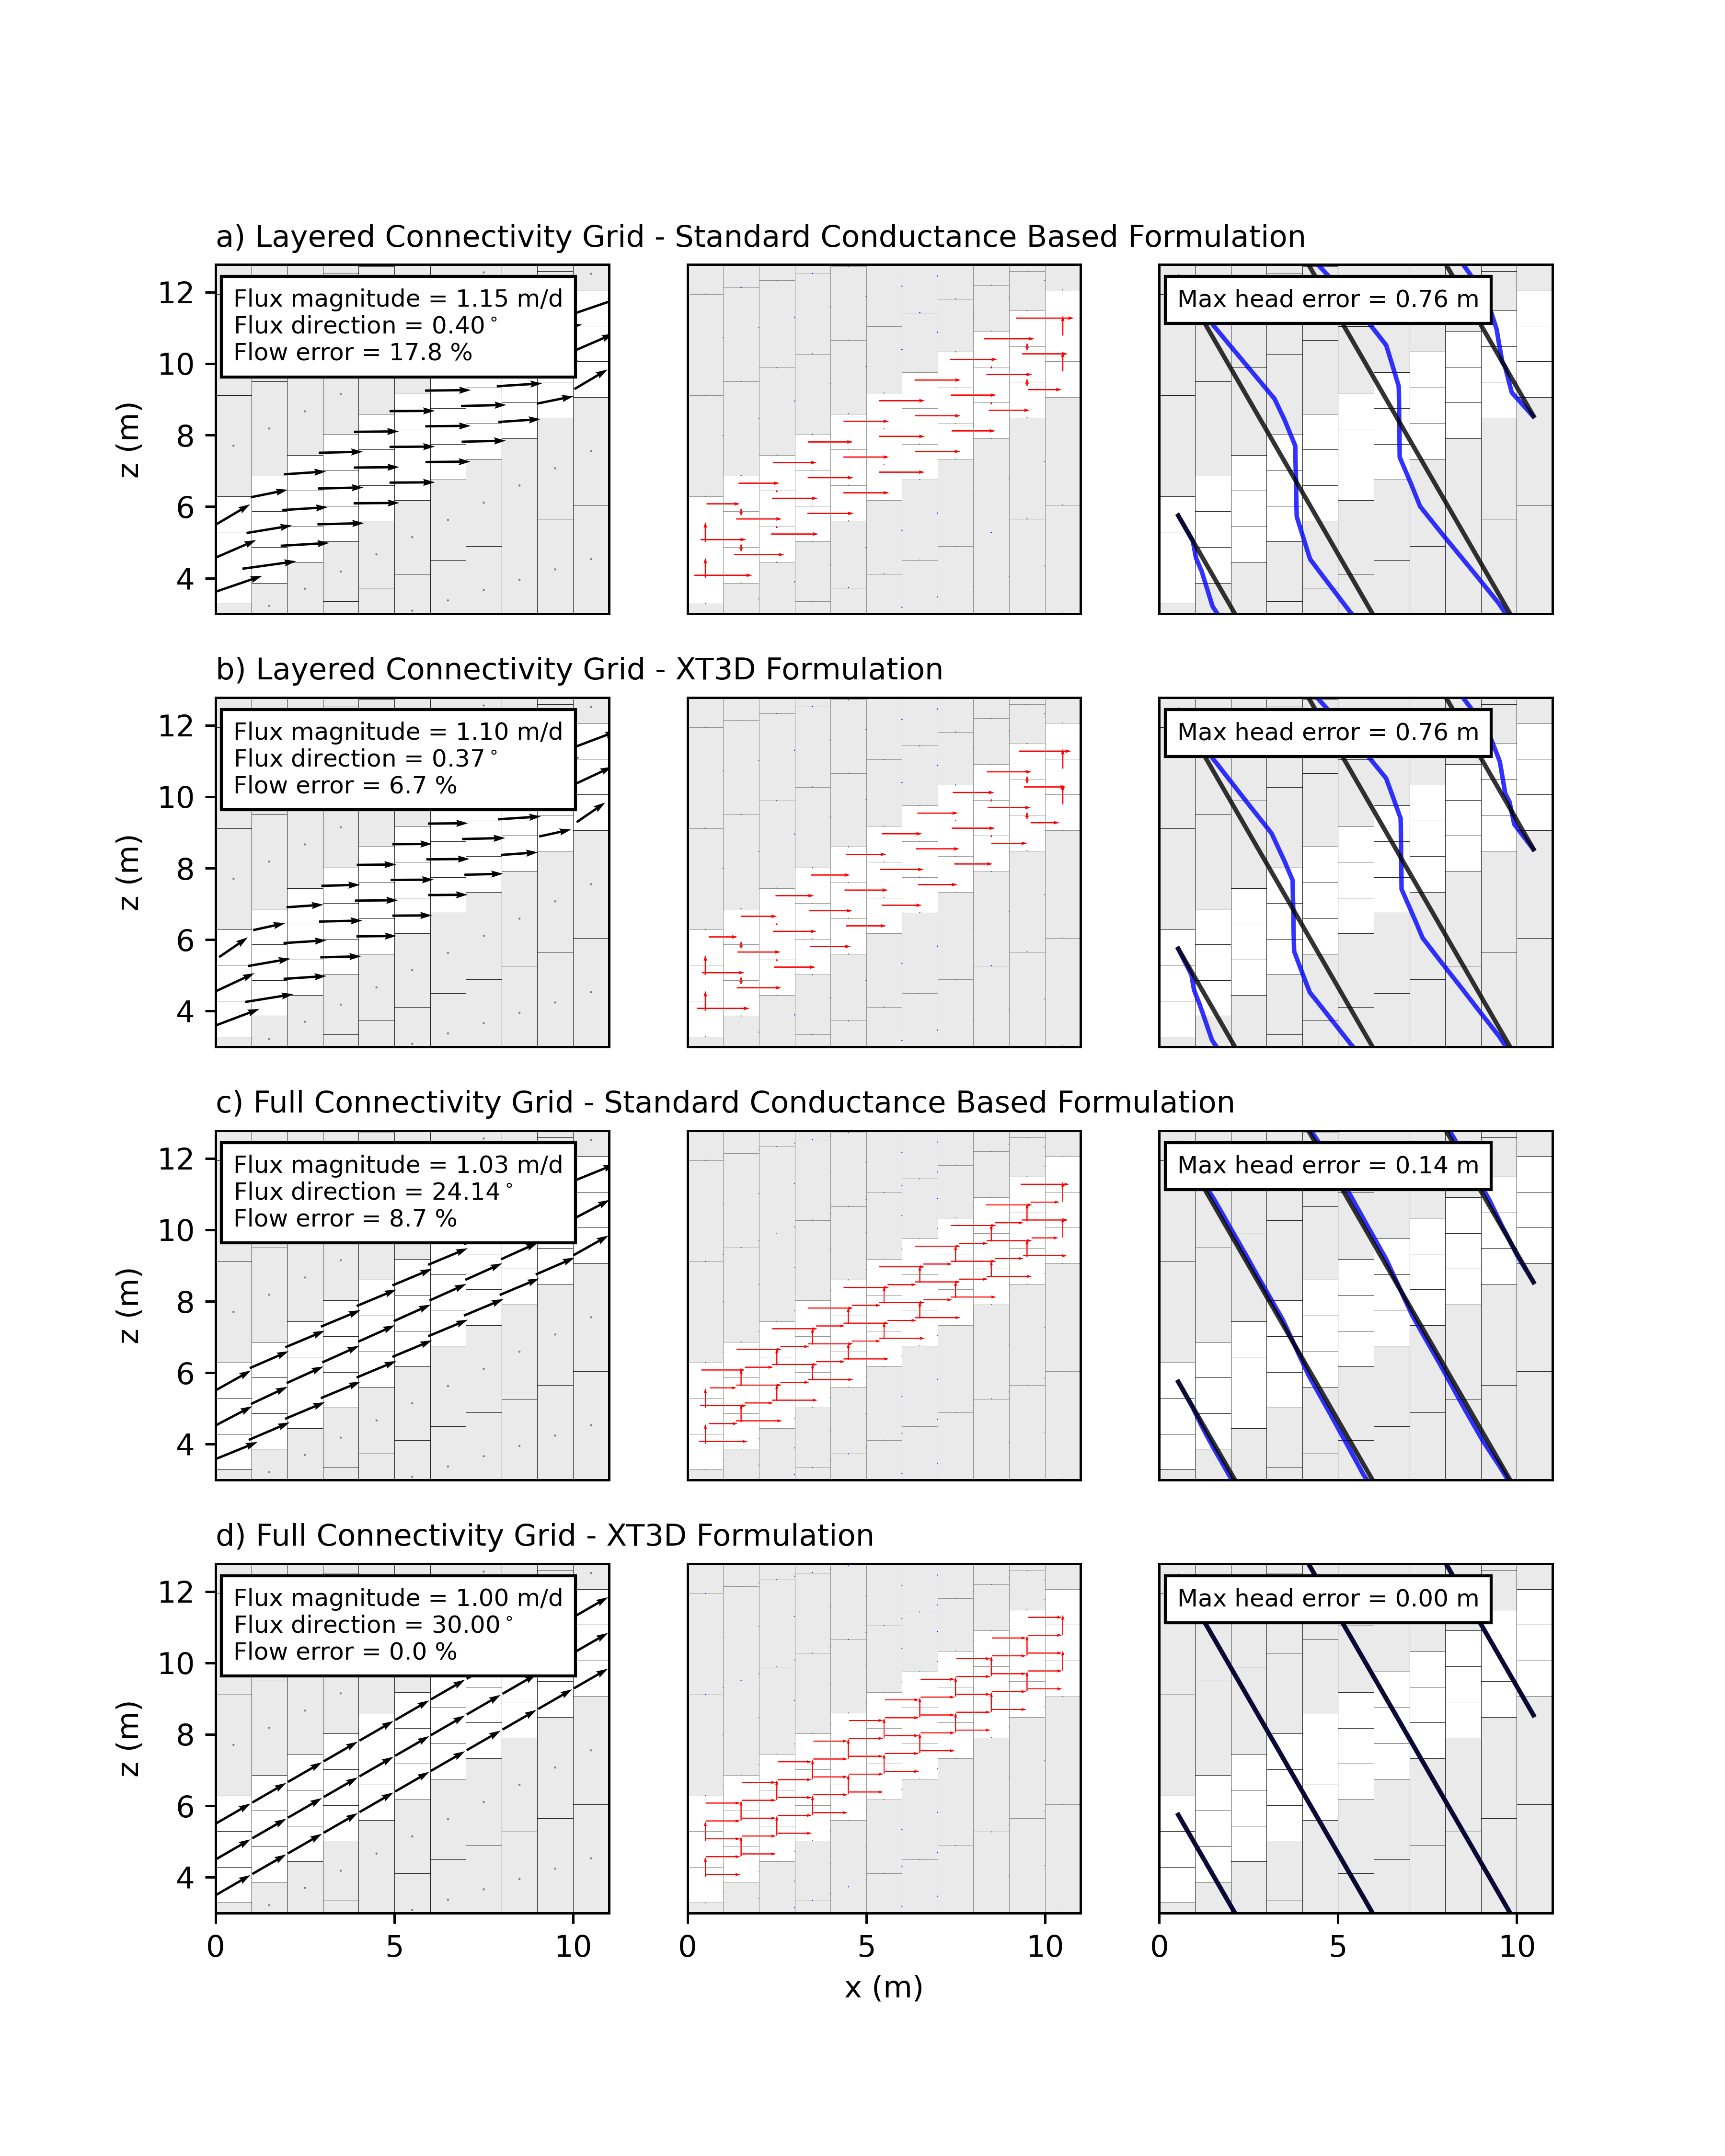
\includegraphics[scale=0.8]{../figures/fig2_paper.png}
	\caption{Numerical results for the test problem using base-case settings for layered-connectivity and full-connectivity grids, with the standard conductance based formulation as well as the XT3D formulation. The left panel of each scenario shows the calculated specific discharge at each cell centre within the aquifer (black arrows) and domain (grey arrows). The middle panel shows the face flows (red arrows). The right panel shows head contours for the analytical solution (black) as well as the numerical solution (blue).}
	\label{fig:fig2}
	\end{center}
\end{figure}

\subsection{Effects of Grid Resolution}

\begin{figure}
	\begin{center}
	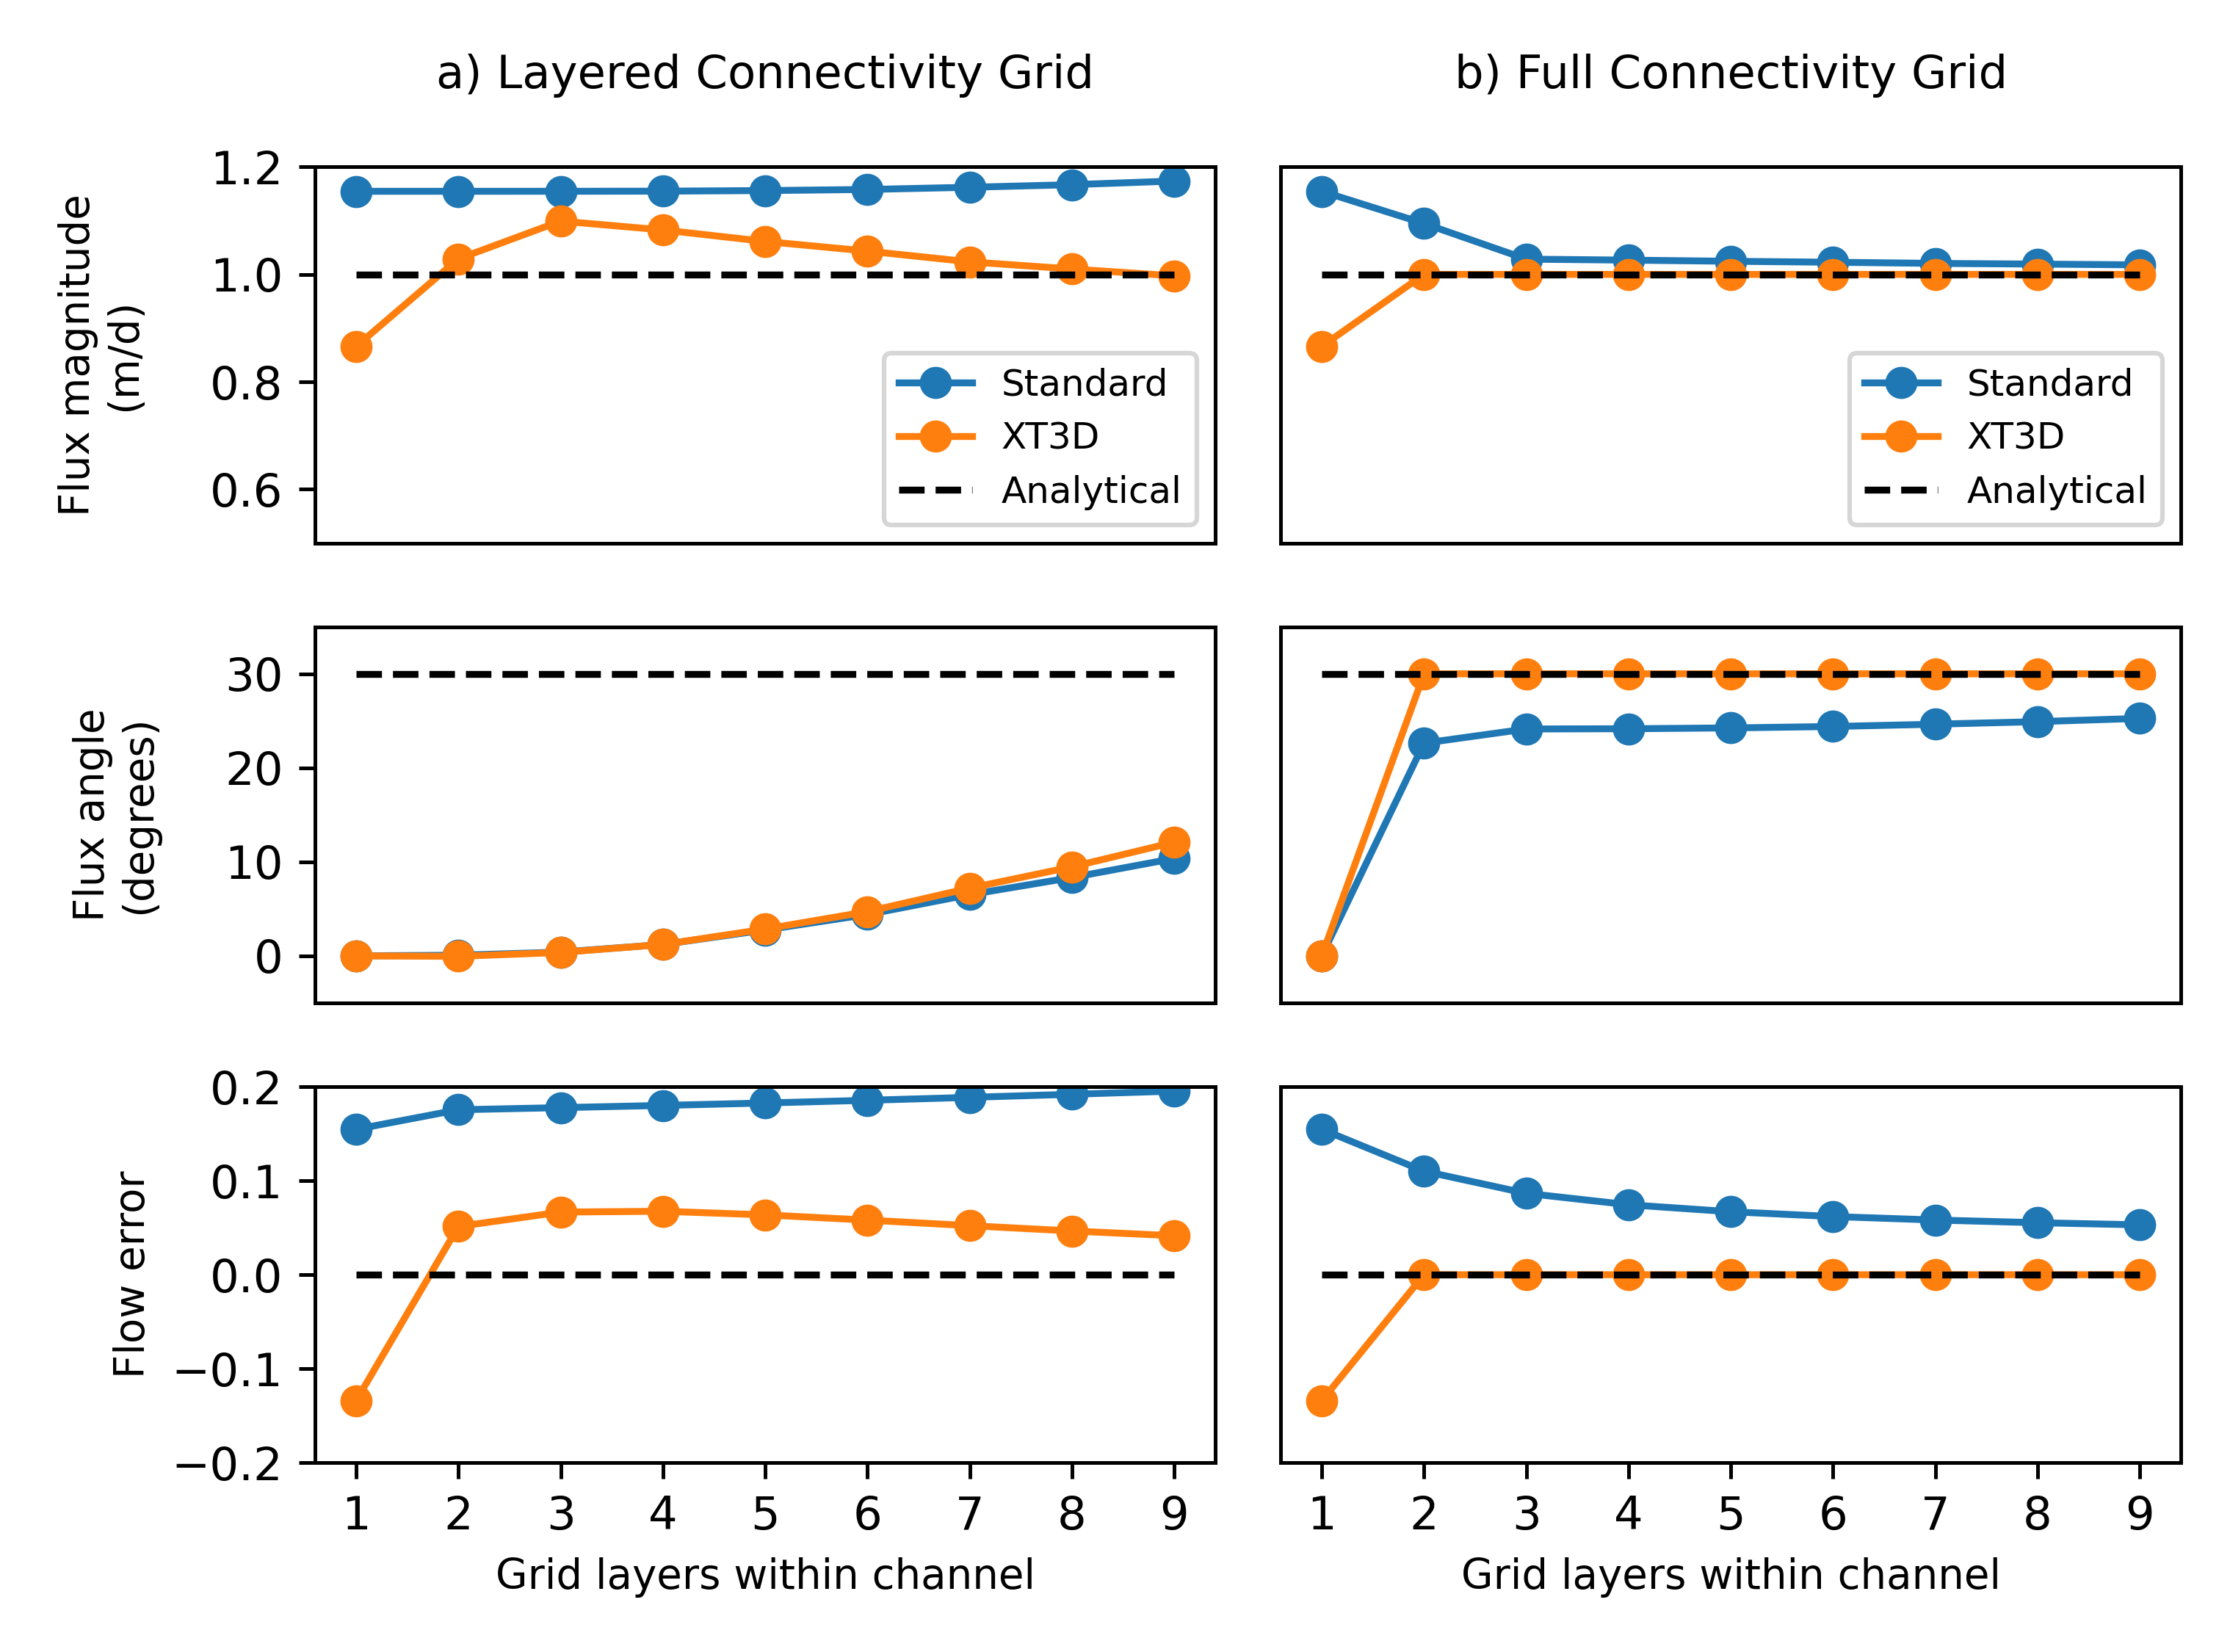
\includegraphics[scale=0.9]{../figures/fig3paper.png}
	\caption{Graphs indicating how increasing the number of grid layers within a single hydrogeologic layer (in this case, the aquifer) affects flux magnitude of middle cell (top), flux direction of middle cell (middle) and volumetric flow through the hydrogeologic layer (bottom). We immediately notice the errors layered-connectivity grids incur (left panel), and how using a full-connectivity grid (right panel), particularly in conjunction with XT3D (orange line) reproduces the analytical solution from two grid layers used to discretize the hydrogeologic layer.}
	\label{fig:fig3}
	\end{center}
\end{figure}

The base case arbitrarily uses 3 grid layers to represent the aquifer, but it is important to address the question: \emph{How many grid layers are required to adequately represent a hydrogeological layer?}. Layered-connectivity grids, which are commonly used by groundwater modelers \citep{Reilly2004}, are almost always configured as one grid layer per hydrogeological unit when simulating groundwater flow. {\color{red} (AMP: Could maybe mention that it's generally well known you want multiple layers for accurate transport? JM: Added "when simulating groundwater flow" to just specify flow explicitly and keep things simple)} However, although computationally efficient, we investigate the effect of altering resolution within the aquifer by using the base case and varying number of cells per aquifer width from one to nine (Figure \ref{fig:fig3}). When increasing resolution, cells inside the aquifer were maintained as a square shape to allow fair comparison between models of varying refinement, uncomplicated by cell distortion. Therefore, the height of the model extended as each additional grid layer was added to represent the aquifer. We compare modeled flux magnitude and direction in the center cell, as well as volumetric flow against the analytical solution. 

Flux magnitude error for layered-connectivity grids peaked at around 10\% but improved and tended to zero with refinement. Flux direction for layered-connectivity grids is clearly a major issue, being reported as horizontal for one grid layer per aquifer width, and only improved to 12$^{\circ}$ for 9 grid layers per aquifer width. Flow through the aquifer peaked at 13\% error but decreased to only a 4\% error for 9 grid layers per aquifer width. 

The results for the full-connectivity grid clearly show that a minimum of two grid layers per aquifer width is required to match the analytical result for flux magnitude, direction and volumetric flow. This is an important finding as it demonstrates that computational efficiency can be made using a full-connectivity grid over a rectilinear grid overlay approach, but it is important to use a minimum of two grid layers per hydrogeological unit to allow vertical fluxes to be incorporated into the flow solution. 

\subsection{Effects of Dip Angle and Conductivity Contrast}

The base case uses a dip angle of 30$^{\circ}$ and an extreme conductivity contrast between aquifer and domain of 1:$10^{-6}$. Here, we investigate the behavior of the flow solution for a wide range of aquifer inclines by systematically changing the dip angle by 2.5$^{\circ}$ from 0 to 80$^{\circ}$. Similarly, we examine the solution for multiple conductivity contrasts by changing the domain conductivity to 2, 5, 10 and 100 times less than the aquifer.  Simulated flux magnitude and direction of the center cell for all combinations are plotted against the analytical solution in Figure 4. 

Traditional layered-connectivity grids without XT3D shows rapid diversion of flux magnitude and direction from the analytical solution as dip increases (Figure 4a). Use of the XT3D option keeps the flux magnitude somewhat on-track until about 30$^{\circ}$ when the solution starts peeling away from the analytical (Figure 4b). Flux direction is improved for the homogeneous scenario, but not for the heterogeneous scenarios. The full-connectivity grid on the other hand, even without XT3D, roughly follows the analytical solution for flux magnitude and direction until around 65$^{\circ}$ when it starts to ``fall-apart'' (Figure 4c). There are also spikes at certain dip angles which are related to transitions between cell connections due to changing cell face overlaps. The full-connectivity grid with XT3D clearly boasts the best results (Figure 4d) with the flux magnitude and direction matching the analytical until 65$^{\circ}$, with the exception of a slight decrease in flux direction after 45$^{\circ}$. The errors reflect the discretization choice of the model. For the 1 m by 1 m cells, the aquifer center cell is fully connected to other aquifer cells up to an angle of 45$^{\circ}$. After 45$^{\circ}$, some aquifer cell faces share greater overlap with domain cell faces than the adjacent aquifer cell face. After 65$^{\circ}$, the aquifer center cell loses all lateral connections to adjacent aquifer cells such that only vertical aquifer connections remain, forcing flow vertically (90$^{\circ}$). To rectify this issue when encountering dips greater than 45$^{\circ}$, and especially after 65$^{\circ}$, finer discretization in the vertical and horizontal directions should be made to maximize inter-aquifer cell connections.  

These results confirm that full-connectivity grids with XT3D not only outperform the alternatives when modelling dipping hydrogeological units, but come extremely close to the analytical solution. We note that these results relate to the chosen discretization. The key element is to ensure that the discretization maintains connectivity at the most extreme angles. {\color{red} (JLM: is the advice here that the ratio of vertical to horizontal dicretisation needs to be approximately $\arctan(\theta)$ for three sub-layers. Could be a general formula for $\theta$ and number of sub cells)}

\begin{figure}[p!]
\centering
\begin{subfigure}{0.9\textwidth}
	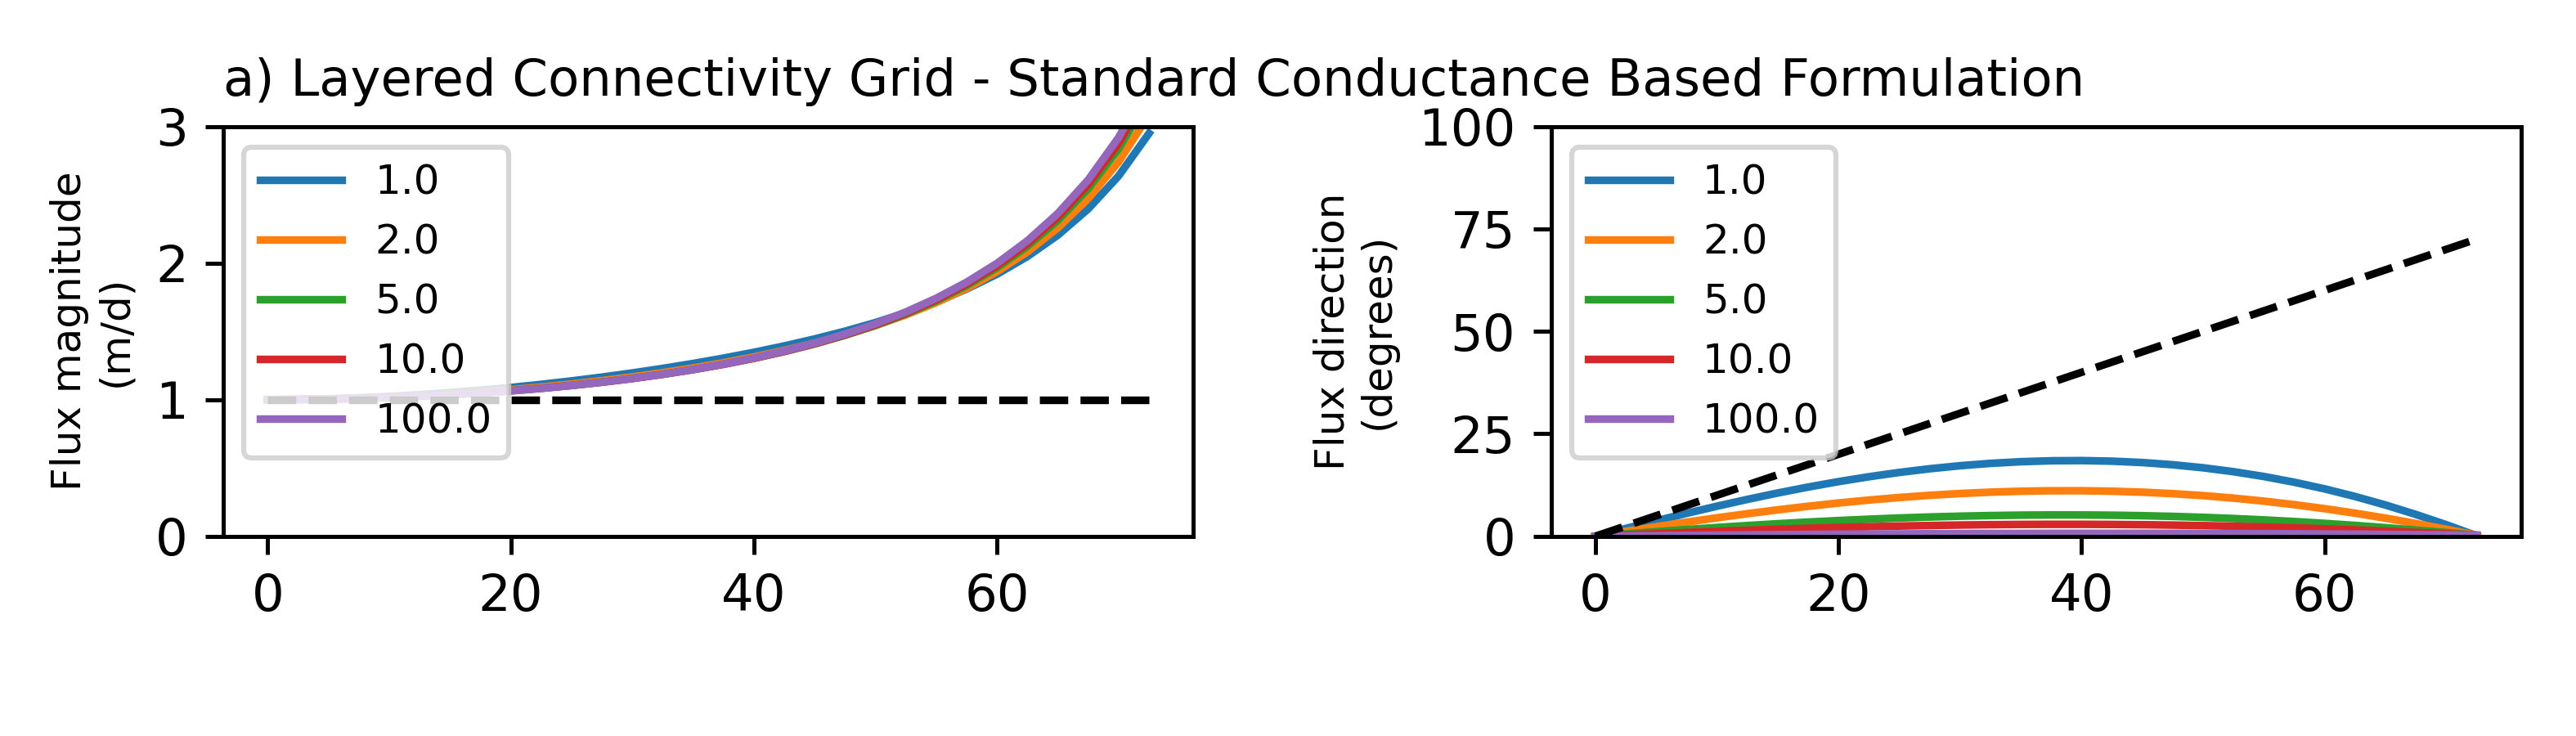
\includegraphics[width=\textwidth]{../figures/fig4_0_paper.png}
\end{subfigure}
\begin{subfigure}{0.9\textwidth}
	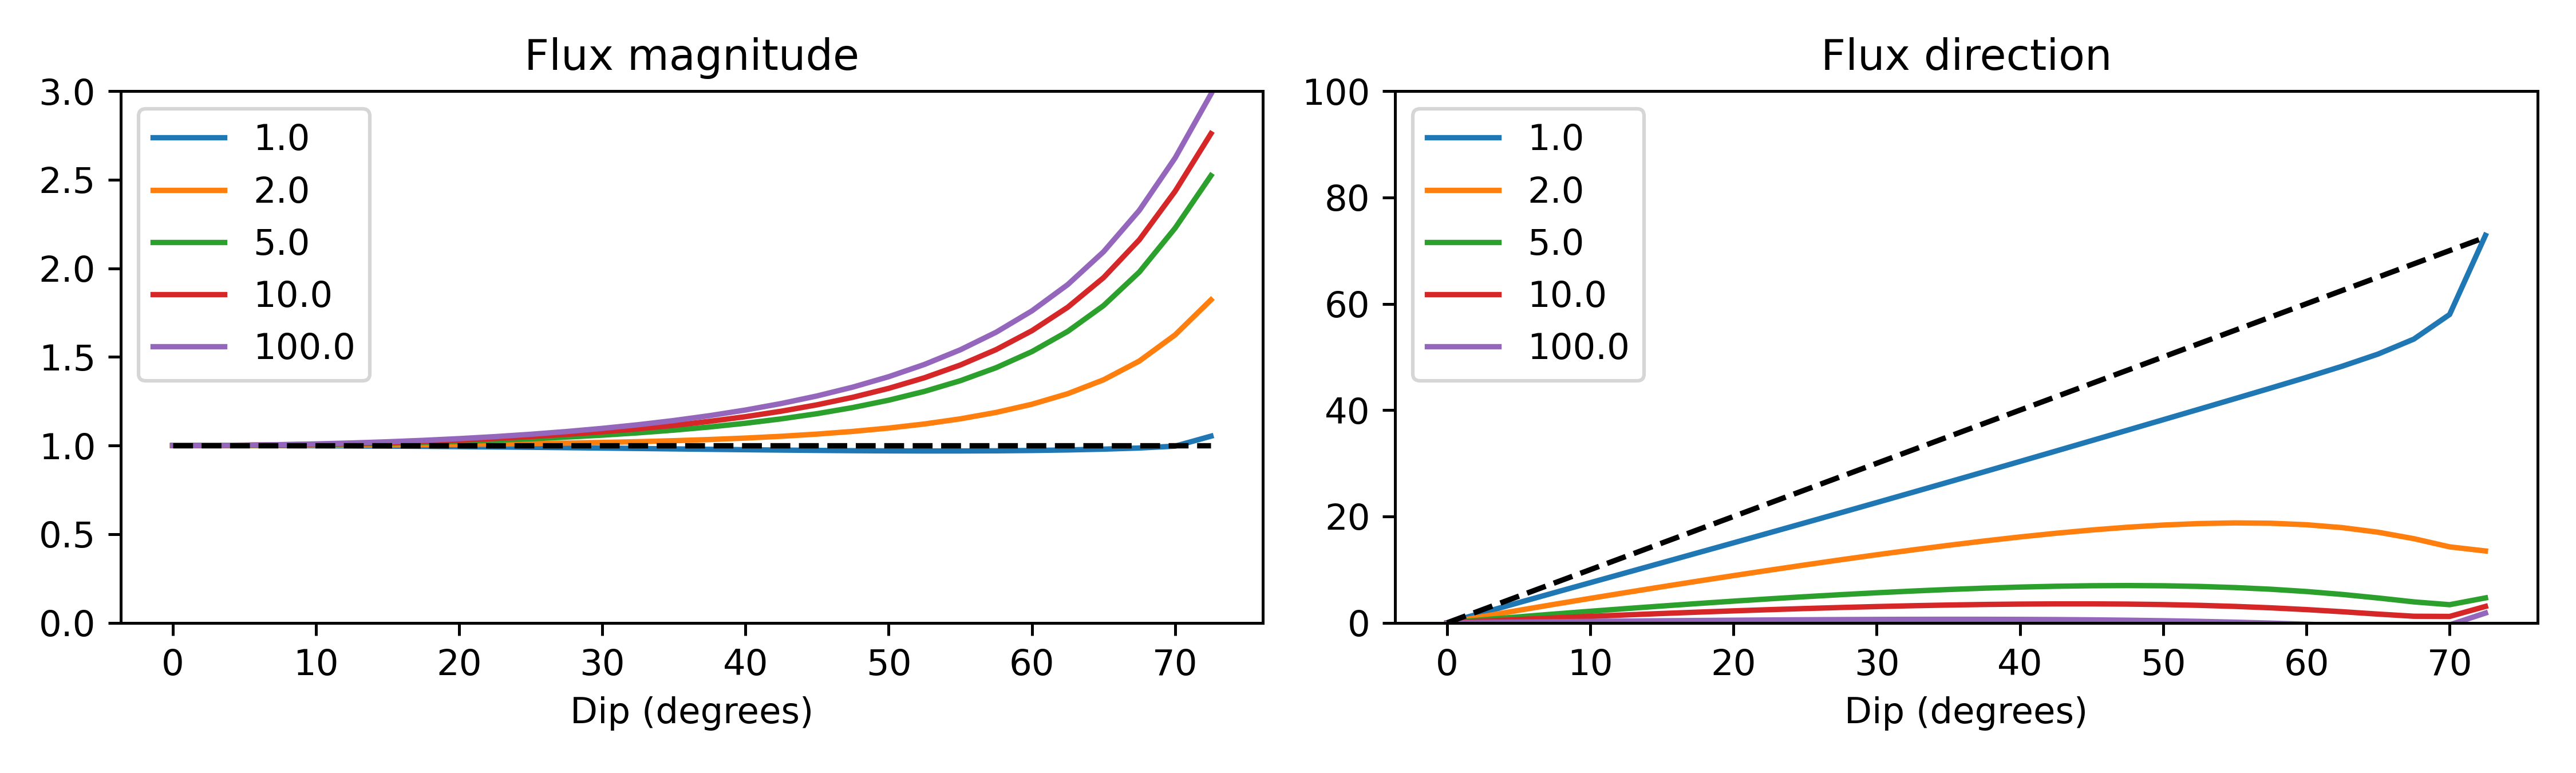
\includegraphics[width=\textwidth]{../figures/fig4_1_paper.png}
\end{subfigure}
\begin{subfigure}{0.9\textwidth}
	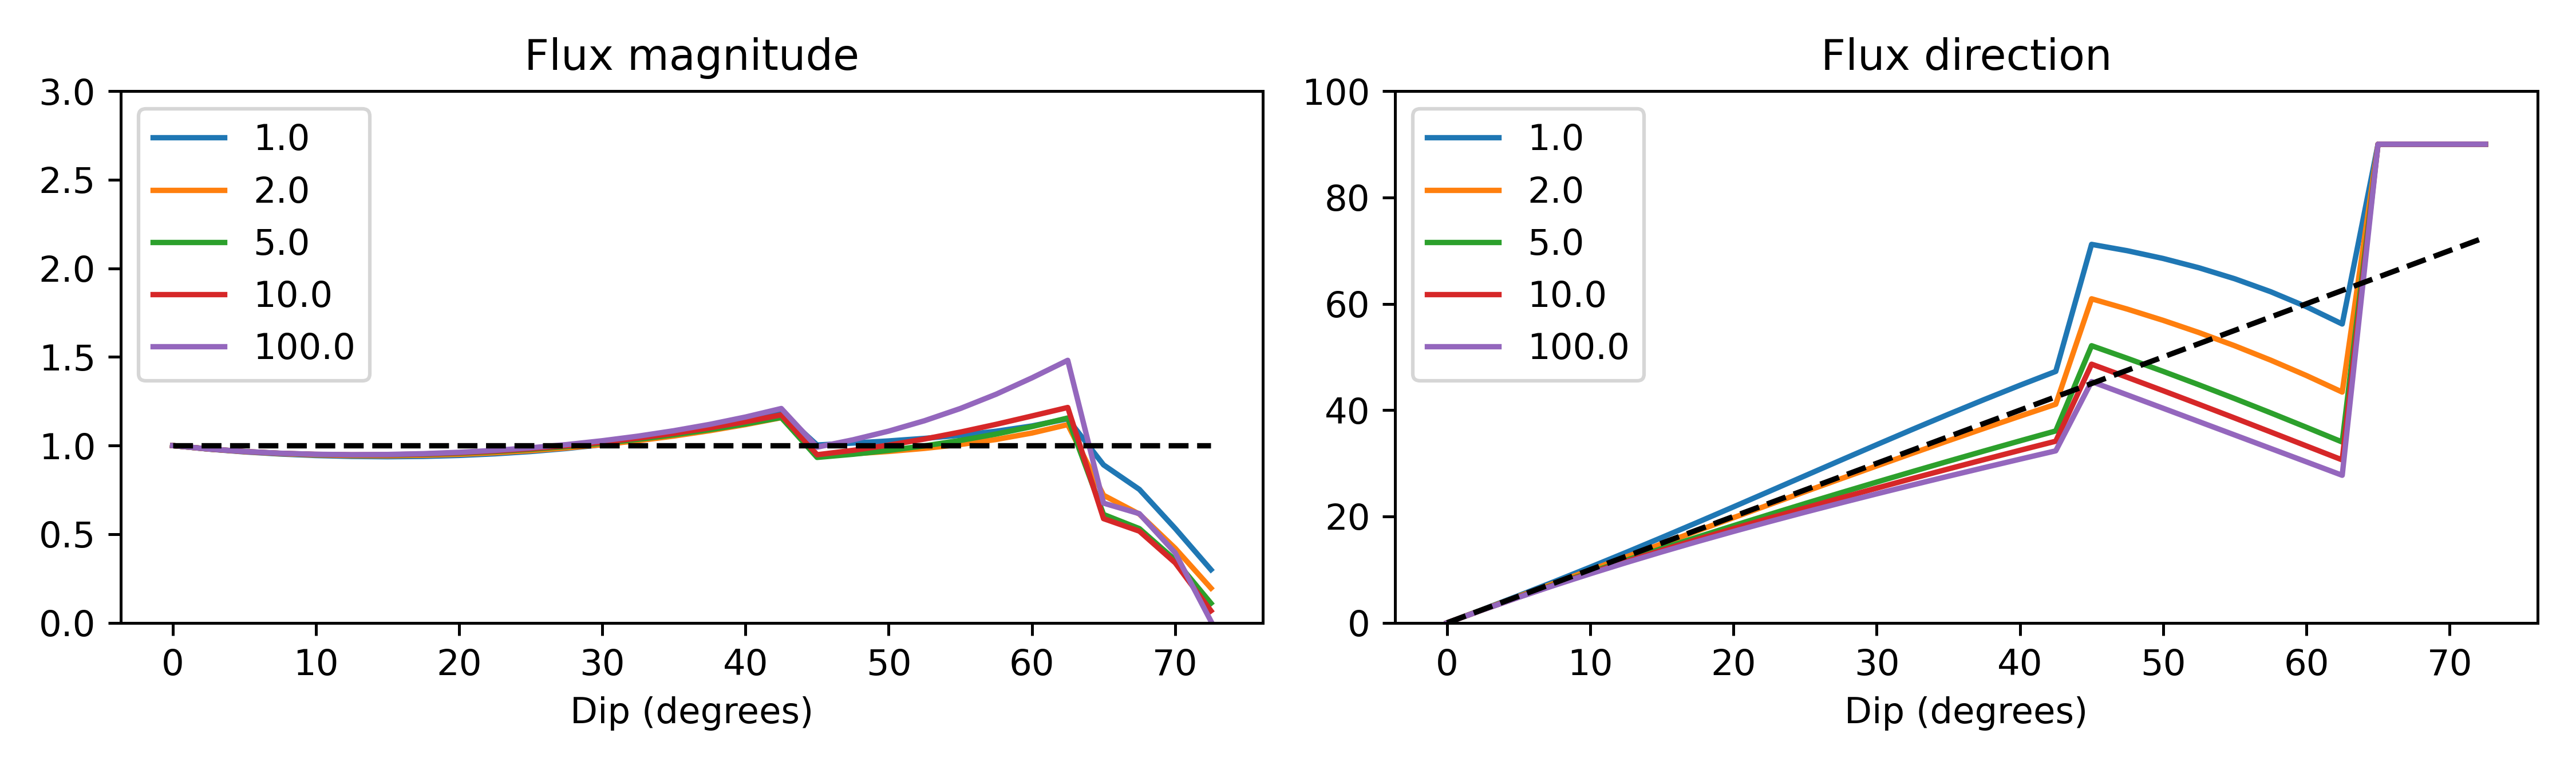
\includegraphics[width=\textwidth]{../figures/fig4_2_paper.png}
\end{subfigure}
\begin{subfigure}{0.9\textwidth}
	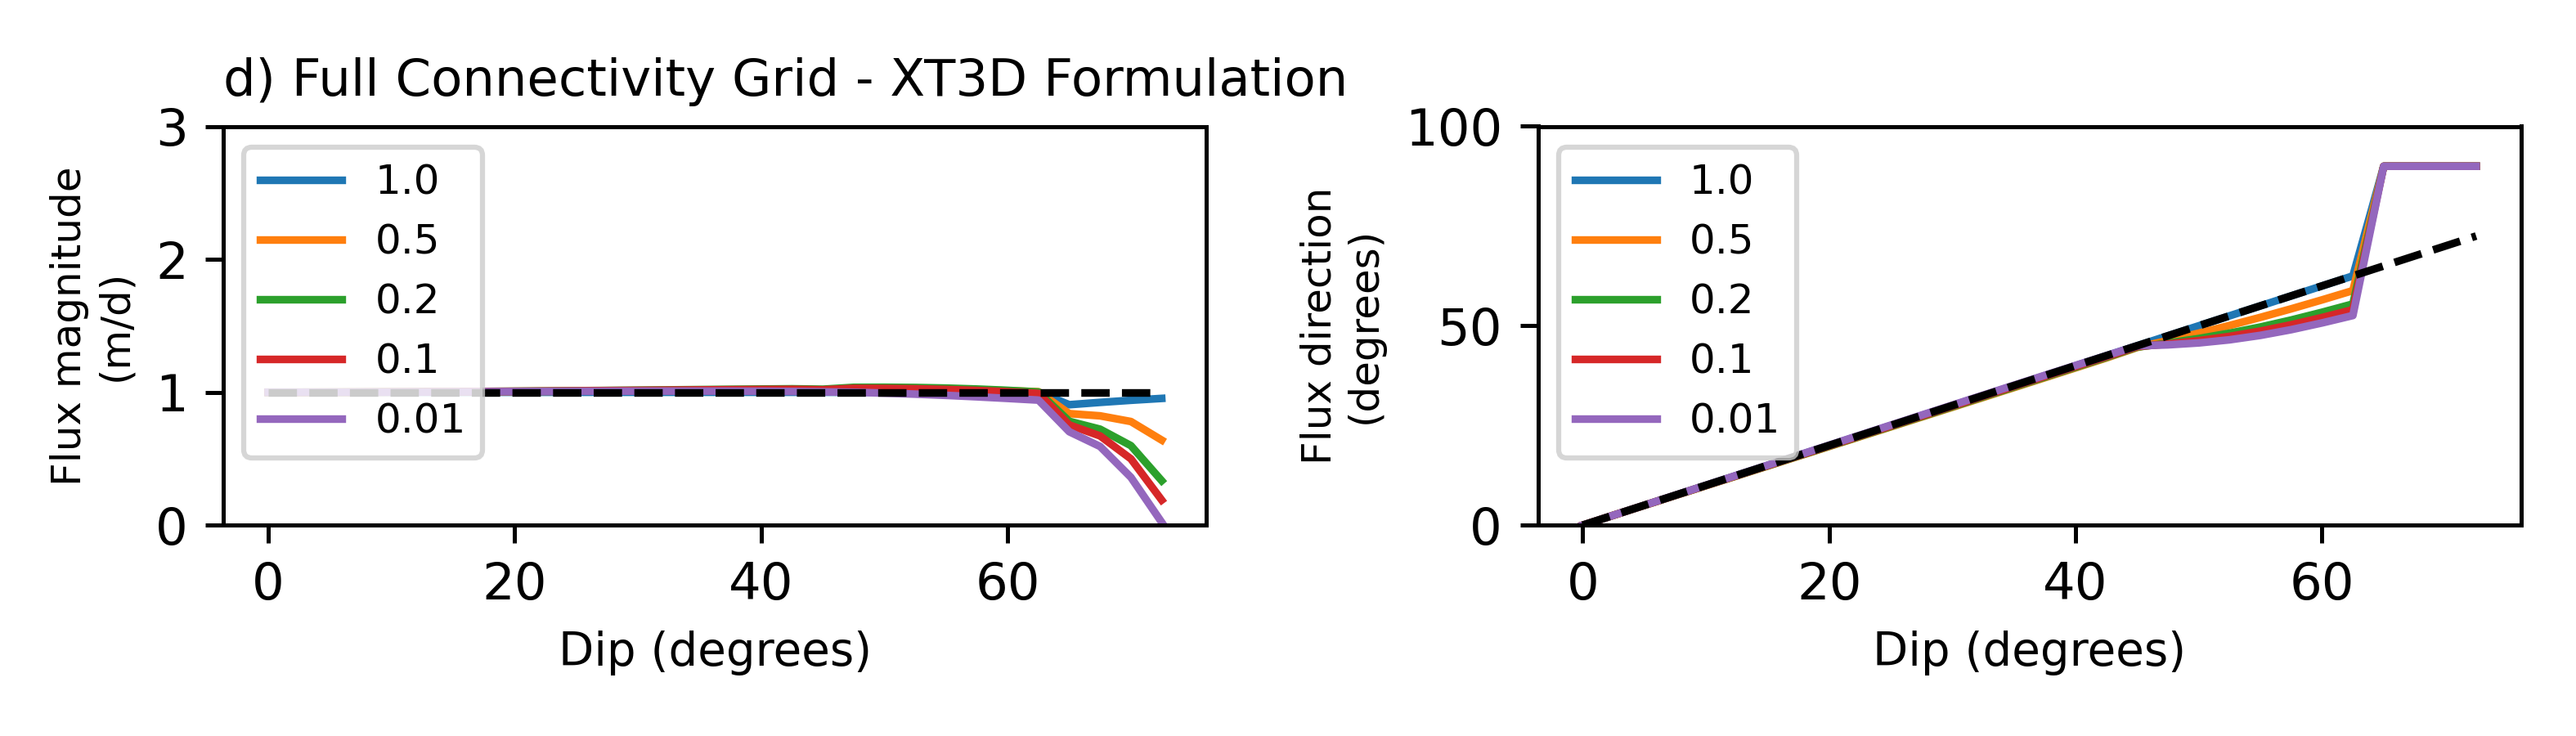
\includegraphics[width=\textwidth]{../figures/fig4_3_paper.png}
\end{subfigure}

\caption{Flux magnitude and direction for centre cells for varying contrasts in log conductivity (blue, orange, green, red lines) for varying dip angles (x-axis). The analytical value is shown in black dashed line.}
\label{fig:figures}
\end{figure}

\subsection{Effect of Anisotropy}

The base case and subsequent scenarios have assumed isotropic conductivity. However, sedimentary layers often exhibit anisotropic conductivity, and therefore we examine the gridding strategies using anisotropic and dipping conductivity tensors within the aquifer, with reduced conductivity perpendicular to the aquifer by 10, 100, 1000 and 10,000. We also include the isotropic scenario (ratio of 1). Results are presented in Figure \ref{fig:fig5}. Layered-connectivity grids produce flux magnitude and flow results that significantly deviate from the analytical solution both with and without the XT3D formulation (Figure \ref{fig:fig5}a), whilst full-connectivity grids with XT3D reproduce the analytical solution (Figure \ref{fig:fig5}b, orange line). These results verify, once again, our proposed method of using full-connectivity grids to model dipping anisotropic hydrogeologic layers.


\begin{figure}
	\begin{center}
	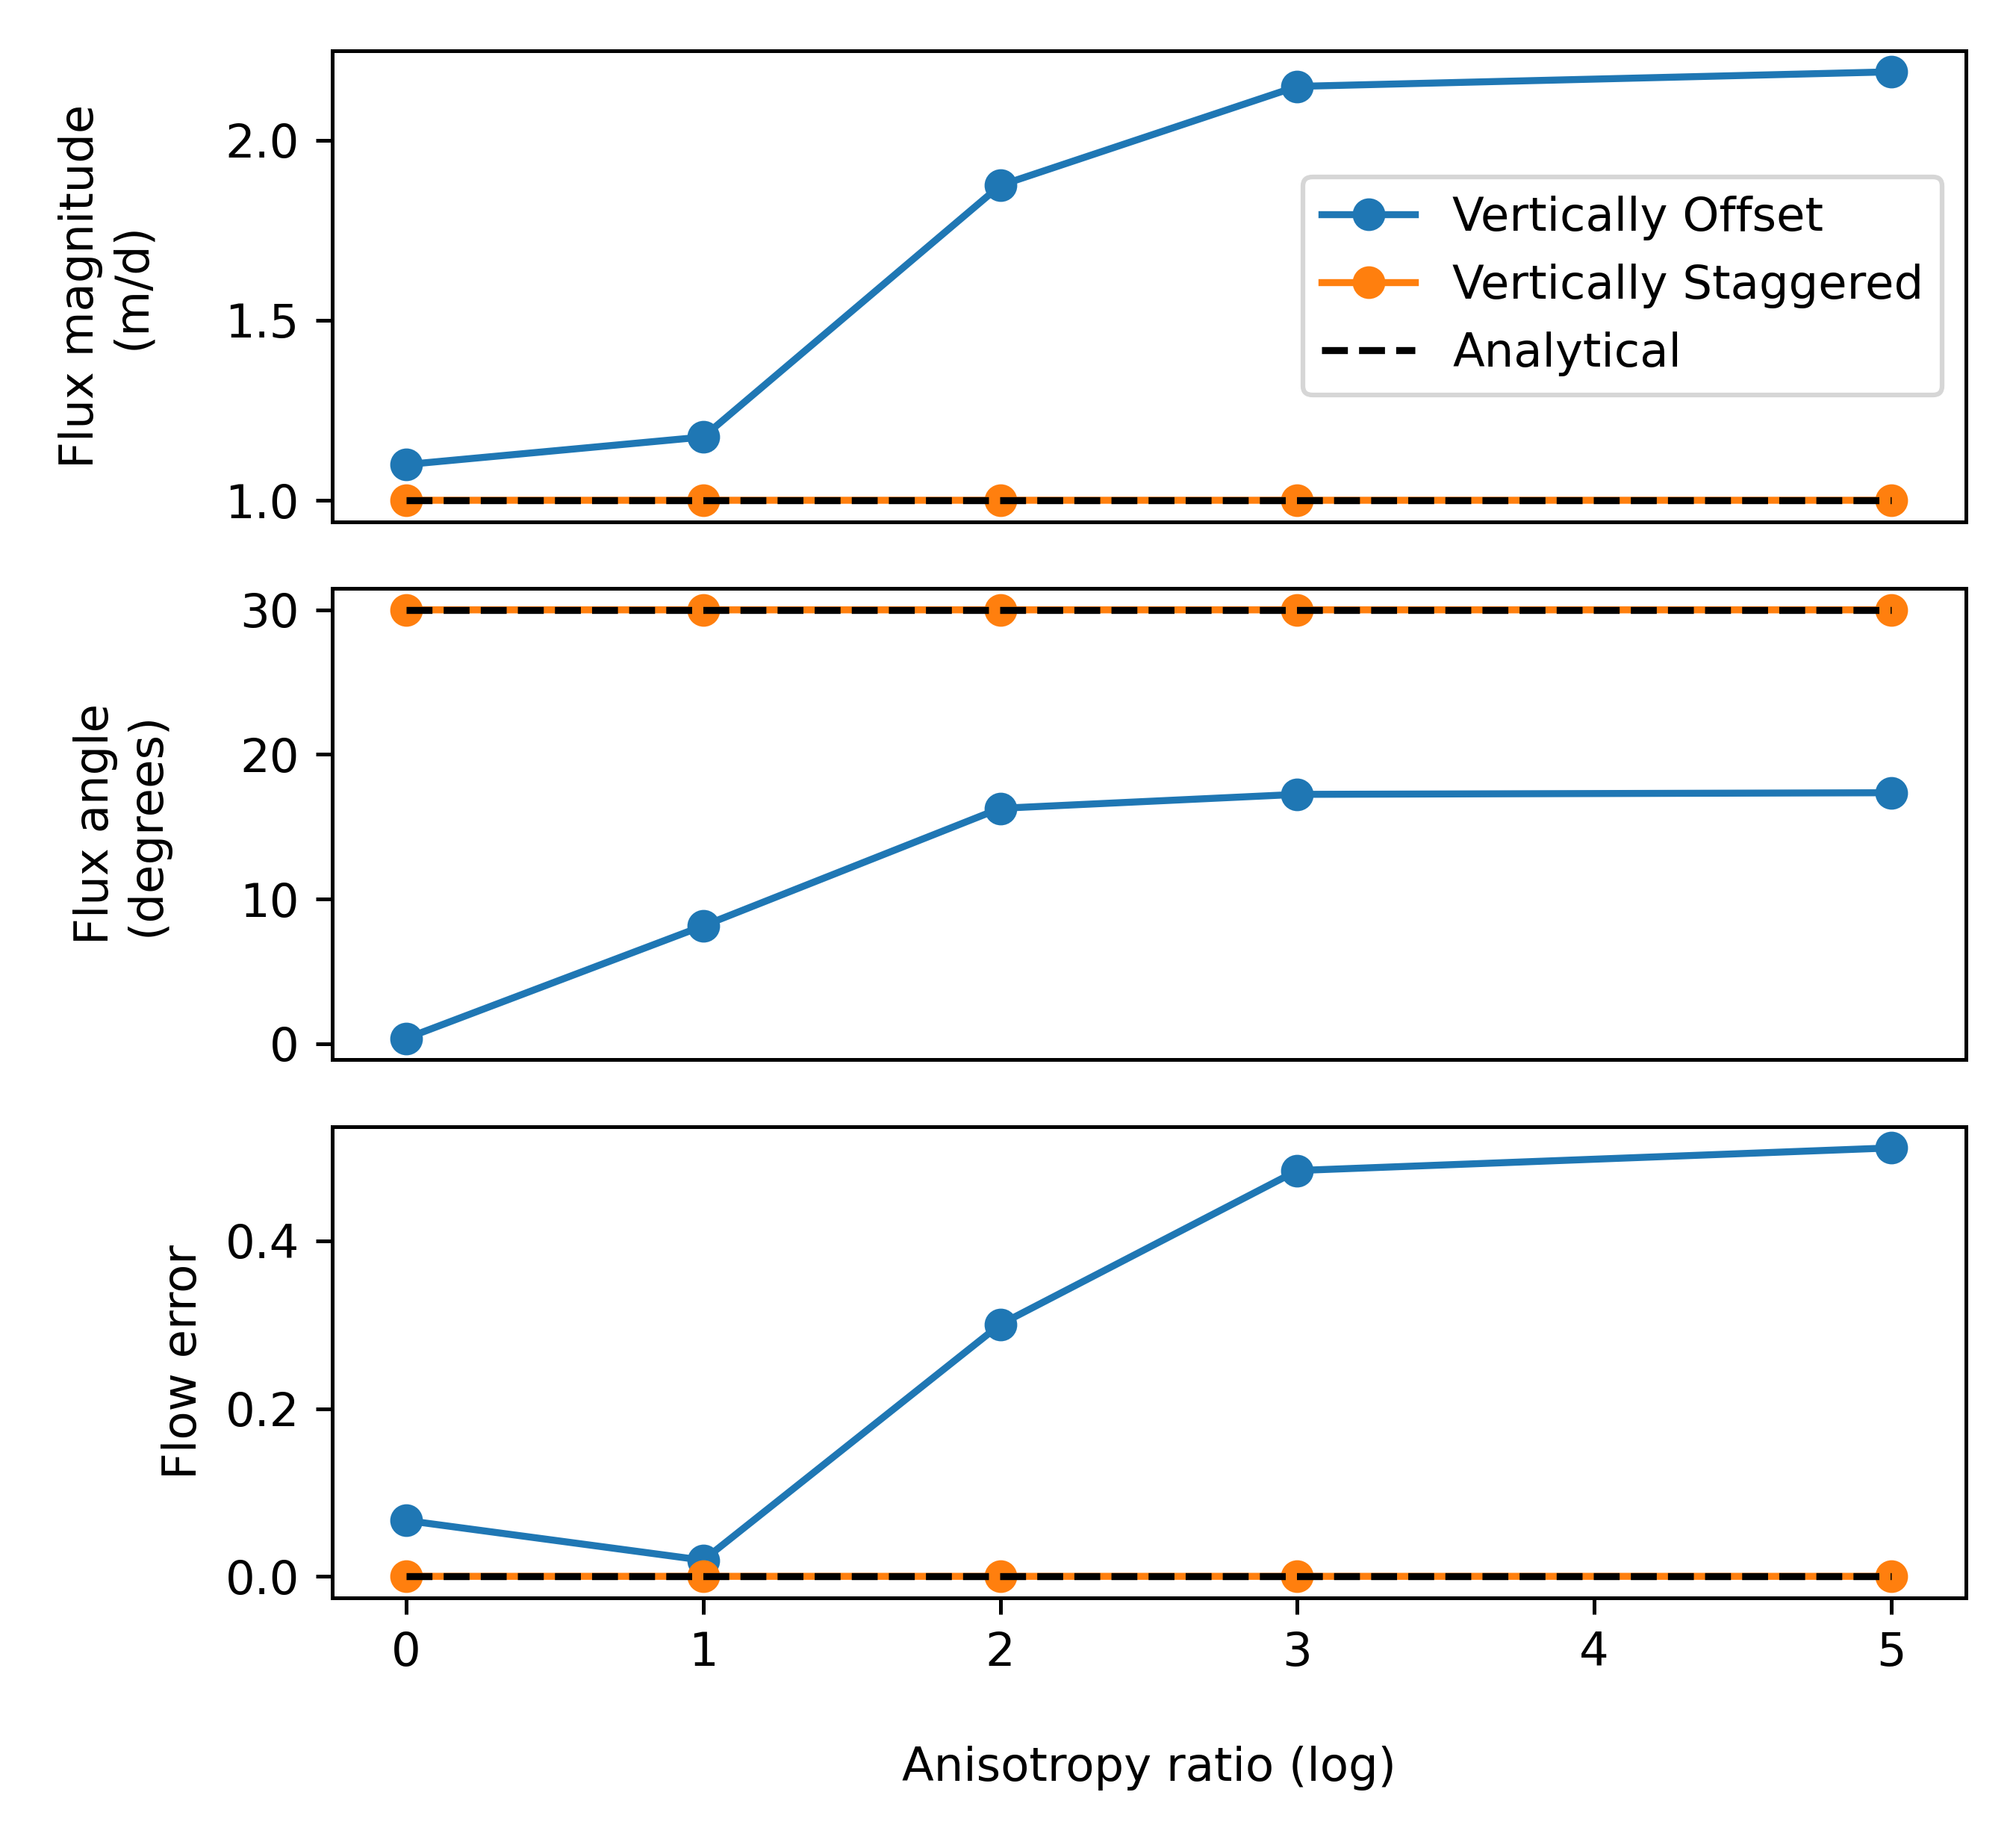
\includegraphics[scale=0.9]{../figures/fig5paper.png}
	\caption{Varying anisotropy ratios of conductivity withing the aquifer and the resulting flux magnitude of middle cell (top panel), flux direction of middle cell (middle panel) and volumetric flow through the aquifer (bottom panel). Plots include results for the standard conductance-based formulation (blue) as well as the XT3D formulation (orange).}
	\label{fig:fig5}
	\end{center}
\end{figure}


\section{Conclusions}

 \cite{bardot2022} revisited the capability of MODFLOW to accurately simulate groundwater flow through sedimentary structures.  They concluded that the XT3D multi-point flux approximation in MODFLOW 6 significantly improves the accuracy of simulated flows when used with a grid-overlay approach in which locations of sedimentary structures, which can be steeply dipping, are mapped onto a relatively fine, rectilinear model grid.  They also concluded that the XT3D multi-point flux approximation does not perform as well as anticipated when simulating flow through a steeply dipping hydrogeologic layer using deformed vertically offset grids, which are advantageous for significantly reducing the number of grid layers required for many problems.  They hypothesized that the inherently limited lateral connectivity between cells in DIS and DISV layered grids in MODFLOW 6 was responsible for the inability to obtain accurate flow results in their steeply dipping test problems using vertically offsets grids, with or without XT3D.

In this paper, we have confirmed that the layered lateral connectivity implemented in DIS and DISV model grids is inadequate for simulating groundwater flow through steeply dipping sedimentary structures, even when the XT3D multi-point flux approximation is used.  However, when connections between laterally adjacent cells in different grid layers are added to comprise a grid with full connectivity, there is a substantial increase in the accuracy of simulated flows.  The additional connectivity is implemented using the fully unstructured (DISU) grid type.  Importantly, this accuracy improvement requires that at least two grid layers be used to represent the dipping aquifers, with additional grid layers required for very steep dips above 65$^{\circ}$.  The primary conclusion of this paper is that, given appropriate discretization and cell connectivity, the XT3D multi-point flux approximation implemented in MODFLOW 6 can be combined with vertically offset grids to efficiently and accurately model flows through steeply dipping sedimentary structures.  Prior to this work, the capability to efficiently and accurately model flow through steeply dipping sedimentary structures was generally restricted to finite element simulators.

The importance of adequate connectivity has been explained and evaluated in this work specifically in terms of hydrogeologic layers that correspond to sedimentary structures. However, the impact of cell connectivity on the accuracy of simulated flows should be considered in any MODFLOW application that models flow through a heterogeneous hydraulic conductivity field using a grid with large vertical offsets between laterally adjacent cells, whether or not the grid has a layered structure. The full connectivity needed to improve accuracy can be implemented using the DISU grid types in both MODFLOW 6 and MODFLOW-USG.



\section{Acknowledgments}
We would like to acknowledge.... {\color{red} that this paper is almost ready to GO!! Yeeeha!}

\section{Supporting Information}

\section{Appendix}

\bibliography{references.bib}


\end{document}
